\documentclass{article}

% Global layout
\usepackage%
[
        a4paper,
        % left=2cm,
        % right=2cm,
        % top=2cm,
        % bottom=2cm,
        % vmargin=2cm % vertical margins
        % hmargin=3cm % horizontal margins
        margin=3cm
]
{geometry}
\usepackage{fancyhdr, graphicx, hyperref, indentfirst, lastpage, setspace}

% Encoding
\usepackage[utf8]{vntex, inputenc}
\usepackage[english]{babel}
\usepackage{amsmath, amssymb, gensymb, textcomp}

%%%%%%%%%%%% Bibliography %%%%%%%%%%%%
\usepackage[english]{babel}
\usepackage[backend=biber,style=alphabetic,sorting=ynt]{biblatex}
\usepackage{csquotes}

% Better table
\usepackage{array, booktabs, multicol, multirow, siunitx, tabularx}
% Wide tables go here https://tex.stackexchange.com/questions/332902/my-table-doesnt-fit-what-are-my-options

% Better enumerate
\usepackage{enumitem}

%%%%%%%%%%%% Code space %%%%%%%%%%%%
\usepackage[dvipsnames]{xcolor}
\usepackage{tikz}
\usepackage[framemethod=tikz]{mdframed}
\usepackage{minted, verbatim} % needs python Pygments and --shell-escape flag

% Graphics
\usepackage{caption, float}

% Bibliography
\addbibresource{ref.bib} % references file
\nocite{*} % include all entries in references section

% Page setup
\allowdisplaybreaks{} % to have page breaks inside align* environment
\hypersetup{urlcolor=blue,linkcolor=black,citecolor=red,colorlinks=true}
\numberwithin{equation}{section}
\usemintedstyle{emacs} % pygment/code color format
\renewcommand{\arraystretch}{1.2} % space between table rows

% Global style setup
\makeatletter % change font size for not having underfull hbox
\renewcommand\Huge{\@setfontsize\Huge{22pt}{18}}
\makeatother

\AtBeginDocument{\renewcommand*\contentsname{Contents}}
\AtBeginDocument{\renewcommand*\refname{References}}
\setlength{\headheight}{40pt}

\pagestyle{fancy}
\fancyhead{} % clear all header fields
\fancyhead[L]{
  \begin{tabular}{rl}
    \begin{picture}(25,15)(0,0)
    \put(0,-8){
\includegraphics[width=8mm, height=8mm]{./assets/hcmut.png}}
    \end{picture}
    \begin{tabular}{l}
      \textbf{\bf \ttfamily University of Technology, Ho Chi Minh City}\\
      \textbf{\bf \ttfamily Faculty of Computer Science and Engineering}
    \end{tabular}
  \end{tabular}
}
\fancyhead[R]{
	\begin{tabular}{l}
		\tiny \bf \\
		\tiny \bf
	\end{tabular}  }
\fancyfoot{} % clear all footer fields
\fancyfoot[R]{\scriptsize \ttfamily Page {\thepage}/\pageref{LastPage}}
\renewcommand{\headrulewidth}{0.3pt}
\renewcommand{\footrulewidth}{0.3pt}
\newenvironment{code}[1]
{\VerbatimEnvironment%
  \begin{mdframed}[leftline=false,rightline=false,backgroundcolor=magenta!10,nobreak=false]%
    \begin{minted}[linenos=true,breaklines,breaksymbolleft=,obeytabs=true,tabsize=2]{#1}%
}
{
    \end{minted}%
  \end{mdframed}%
} % TODO Sample codeblock

\begin{document}

\begin{titlepage}
  \begin{center}
    VIETNAM NATIONAL UNIVERSITY, HO CHI MINH CITY \\
    UNIVERSITY OF TECHNOLOGY \\
    FACULTY OF COMPUTER SCIENCE AND ENGINEERING
  \end{center}

  \vspace{1cm}

  \begin{figure}[H]
    \centering
    
\includegraphics[width=0.5\textwidth]{./assets/hcmut.png}
  \end{figure}

  \vspace{1cm}

  \begin{center}
    \begin{tabular}{c}
      \textbf{\Large Computer Networks Lab (CO3094)} \\
      {}                                             \\
      \midrule                                       \\
      \textbf{\Large Report (Semester 211)}          \\
      {}                                             \\
      \textbf{\Huge COMPUTER NETWORK DESIGN}         \\
      \textbf{\Huge FOR BUILDING OF A BANK}          \\
      {}                                             \\
      \bottomrule
    \end{tabular}
  \end{center}

  \vspace{3cm}

  \begin{table}[h]
    \begin{tabular}{rll}
      \hspace{1cm} Advisor: & Mr.\ Nguyễn Lê Duy Lai &         \\
                            &                                  \\
      Students:             & Nguyễn Thanh Ngân      & 1911667 \\
                            & Phạm Nhựt Huy          & 1952059 \\
                            & Nguyễn Hoàng           & 1952255 \\
    \end{tabular}
  \end{table}

  \begin{center}
    {\footnotesize HO CHI MINH CITY, NOVEMBER 2021} \\
  \end{center}
\end{titlepage}

%\thispagestyle{empty}

\tableofcontents
\newpage

\section{Requirement Analysis}
\subsection{Requirements}
\subsubsection{Functional requirements}
% TODO

\subsubsection{Non-functional requirements}
% TODO

\subsection{Survey Checklist}
\subsubsection{Headquarters}
% TODO

\subsubsection{Branches}
% TODO

\subsection{Network Structure}
% TODO

\subsection{High Load Areas}
% TODO

\subsection{Wireless Coverage}
% TODO


\section{Network Blueprint}
\subsection{Recommended Equipment}
The following choice of hardware is based on the devices available in Cisco Packet Tracer.
\subsubsection{Router: CISCO2911/K9 }
\begin{itemize}
    \item Quantity: 3
    \item Specification: 3 Gigabit Ethernet Port, 4 Serial Port, 4 Fast Ethernet Port
    \item Ethernet connects the switches and routers in the same area
    \item Serial connects to devices in other areas
\end{itemize}
\begin{figure}[H]
    \centering
    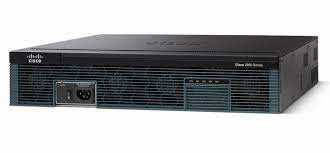
\includegraphics[width=0.6\textwidth]{./assets/router.png}
    \caption{Router CISCO2911/K9}
\end{figure}

\subsubsection{Switches: 2960 24TT}
\begin{itemize}
    \item Quantity: 17
    \item Specification: 24 Fast Ethernet Port, 2 Gigabit Ethernet Port
    \item To provide the DHCP services, each headquarter or branch will need 1 switch
    \item For headquarter, we need 5 switches for 100 workstations
    \item For branches, we need 3 switches for each branch correspond to 50 workstations
    \item A switch at each branch or headquarter to connect the servers to router
\end{itemize}

\begin{figure}[H]
    \centering
    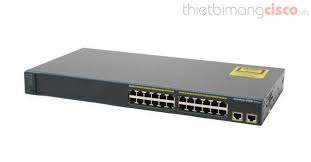
\includegraphics[width=0.7\textwidth]{./assets/switch.png}
    \caption{Switch 2960 24TT}
\end{figure}

\subsubsection{Access point: WRT300N}
\begin{itemize}
    \item Quantity: 3
    \item Specification: 2.4GHz channel WPA2-PSK built-in DHCP server

    \item Provide wireless connection through WPA-PSK authentication
\end{itemize}

\begin{figure}[H]
    \centering
    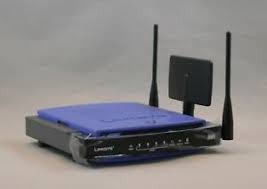
\includegraphics[width=0.5\textwidth]{./assets/wireless_router.png}
    \caption{Access point WRT 300N}
\end{figure}

\subsubsection{DHCP Server}
\begin{itemize}
    \item Quantity: 3
    \item Specification: Static IP procide DHCP service.
\end{itemize}

\subsubsection{Server}
\begin{itemize}
    \item Quantity: 11
    \item Specification: 5 servers for Headquarter, 3 for each branch
\end{itemize}

\subsubsection{Cables}
\begin{figure}[H]
    \centering
    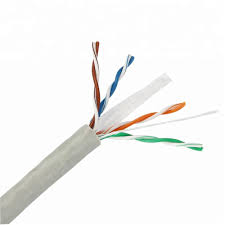
\includegraphics[width=0.4\textwidth]{./assets/copper.png}
    \caption{Straight-through copper cable}
\end{figure}

\begin{figure}[H]
    \centering
    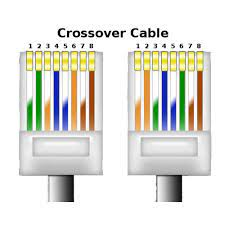
\includegraphics[width=0.4\textwidth]{./assets/crossover.png}
    \caption{Crossover copper cable}
\end{figure}

\begin{figure}[H]
    \centering
    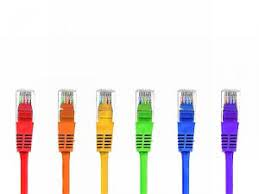
\includegraphics[width=0.6\textwidth]{./assets/lease.png}
    \caption{Leased line cable}
\end{figure}

\subsection{IP Address Table}
\subsubsection{Headquarter}
\begin{center}
  \begin{tabular}{|p{0.06\textwidth}|p{0.2\textwidth}|p{0.15\textwidth}|p{0.15\textwidth}|p{0.15\textwidth}|}
  \hline
   VLAN & Dept & Network ID & Default Gateway & Internet side IP\\
   \hline
   10 & IT/Work Station & 10.0.10.0/24 & 10.0.10.1/24 & 200.0.0.1/30 \\
   \hline
   50 & IT/Server & 10.0.50.0/24 & 10.0.50.1/24 & 200.0.0.1/30\\
   \hline
   N.A & IT/Wireless & 192.168.0.0/24 & 192.168.0.1/24 & 10.0.1.2/30\\
   \hline
    N.A & HQ Gateway router - Wireless Router
&10.0.1.0/30
&10.0.1.1/30
&200.0.0.1/30
\\
\hline
N.A & HQ Gateway router serial link 0
&10.0.0.1/30
&N.A
&N.A\\
\hline
N.A & HQ Gateway router serial link 1
&10.0.0.5/30
&N.A
&N.A
\\
\hline
   \end{tabular}
\end{center}
\subsubsection{Nha Trang branch}
\begin{center}
  \begin{tabular}{|p{0.06\textwidth}|p{0.2\textwidth}|p{0.15\textwidth}|p{0.15\textwidth}|p{0.15\textwidth}|}
  \hline
   VLAN & Dept & Network ID & Default Gateway & Internet side IP\\
   \hline
   10 & IT/Work Station
&10.1.10.0/24
&10.1.10.1/24
&200.0.1.1/30
 \\
 \hline
 50 & IT/Server
&10.1.50.0/24
&10.1.50.1/24
&200.0.1.1/30
\\
\hline
N.A &     IT/Wireless
&192.168.0.0/24
&192.168.0.1/24
&10.1.1.2/30
\\
\hline
N.A & NT Gateway router - Wireless Router
&10.1.1.0/30
&10.1.1.1/30
&200.0.1.1/30
\\
\hline
N.A & NT Gateway router serial link 0
&10.0.0.2/30
&N.A
&N.A
\\
\hline
   \end{tabular}
\end{center}

\subsubsection{Da Nang branch}
\begin{center}
  \begin{tabular}{|p{0.06\textwidth}|p{0.2\textwidth}|p{0.15\textwidth}|p{0.15\textwidth}|p{0.15\textwidth}|}
  \hline
   VLAN & Dept & Network ID & Default Gateway & Internet side IP\\
   \hline
   10 & IT/Work Station
&10.2.10.0/24
&10.2.10.1/24
&200.0.2.1/30
 \\
 \hline
 50 & IT/Server
&10.2.50.0/24
&10.2.50.1/24
&200.0.2.1/30
\\
\hline
N.A &     IT/Wireless
&192.168.0.0/24
&192.168.0.1/24
&10.2.1.2/30
\\
\hline
N.A & NT Gateway router - Wireless Router
&10.2.1.0/30
&10.2.1.1/30
&200.0.2.1/30
\\
\hline
N.A & NT Gateway router serial link 0
&10.0.0.6/30
&N.A
&N.A
\\
\hline
   \end{tabular}
\end{center}

\section{Network Throughput, Bandwidth and Safety Parameters}
The parameters of the flow and load of the system (about 80\% at peak hours 9h-11h and 15h-16h) can be shared for Headquarter and Branches as follows:
\begin{itemize}
  \item Servers used for updates, web access, database access, ..... The total upload and download capacity is about 500 MB / day.
  \item Each workstation is used for Web browsing, document downloads, customer transactions, ... The total upload and download capacity is about 100 MB / day.
  \item WiFi-connected laptop for customers’ accesses about 50 MB / day.
\end{itemize}

\subsection{Headquarter}
\subsubsection{Server}
The total peak hours time in a days is 3 hours (9h-11h and 15h-16h) and may consume up to 80\%. \\
$$Bandwidth = \, \frac{5*500*0.8}{3*3600}*8 = 1.481Mbps$$
$$Throughput = \, \frac{5*500}{8*3600}*8 = 0.694Mbps$$
\subsubsection{Workstation}
Assume each workstation will work 8 hours a day
$$Bandwidth = \, \frac{100*100*0.8}{3*3600}*8 = 5.926Mbps$$
$$Throughput = \, \frac{100*100}{8*3600}*8 = 2.778Mbps$$
\subsubsection{User}
Assume that the number of customers in one day is about 200 customers, and in peak
time is 150 customers. Also, assume that each user access Wifi 8 hours a day.
$$Bandwidth = \, \frac{150*50}{3*3600}*8 = 5.556Mbps$$
$$Throughput = \, \frac{200*50}{8*3600}*8 = 2.778Mbps$$

\subsubsection{Total}
$$Bandwidth = 1.481+5.926+5.556 = 12.963Mbps$$
$$Throughput = 0.694+2.778+2.778 = 6.25Mbps$$

\subsection{Safety parameters}
To ensure for the next 10 years, we need to consider the rate 20\% per five years. The first 5 years, the number of customer will still not increase and this number will increase in the next 5 years.
$$Bandwidth = 12.963*1.2 = 15.556Mbps$$
$$Throughput =6.25*1.2 = 7.5Mbps$$

\subsection{Branch}
\subsubsection{Server}
The total peak hours time in a days is 3 hours (9h-11h and 15h-16h) and may consume up to 80\%. \\
$$Bandwidth = \, \frac{3*500*0.8}{3*3600}*8 = 0.889Mbps$$
$$Throughput = \, \frac{3*500}{8*3600}*8 = 0.417Mbps$$
\subsubsection{Workstation}
Assume each workstation will work 8 hours a day
$$Bandwidth = \, \frac{50*100*0.8}{3*3600}*8 = 2.963Mbps$$
$$Throughput = \, \frac{50*100}{8*3600}*8 = 1.389Mbps$$
\subsubsection{User}
Assume that the number of customers in one day is about 140 customers, and in peak
time is 70 customers. Also, assume that each user access Wifi 8 hours a day.
$$Bandwidth = \, \frac{70*50}{3*3600}*8 = 2.593Mbps$$
$$Throughput = \, \frac{140*50}{8*3600}*8 = 2.778Mbps$$

\subsubsection{Total}
$$Bandwidth = 0.889+2.963+2.593= 6.445Mbps$$
$$Throughput =0.417+1.389+2.778= 4.584Mbps$$

\subsection{Safety parameters}
To ensure for the next 10 years, we need to consider the rate 20\% per five years. The first 5 years, the number of customer will still not increase and this number will increase in the next 5 years.
$$Bandwidth = 6.445*1.2 = 7.734Mbps$$
$$Throughput =4.584*1.2 = 5.501Mbps$$


\section{Packet Tracer Design}
For the core of the network of the given bank, we use three main routers each for the HQ and the two branches.
Moreover, we use 17 switches to provide intranet access to each device and provide DHCP availability.

We define two VLANs for the entire network:
\begin{itemize}
  \item \textbf{VLAN 10} for workstations
  \item \textbf{VLAN 50} for servers
\end{itemize}

As per requirement, we restrict all wireless devices connected to an AP to be able to ping only the devices connected to the same AP\@.
Moreover, we restrict that all the other devices in the same or different area cannot ping the wireless devices.

\begin{figure}[H]
  \centering
  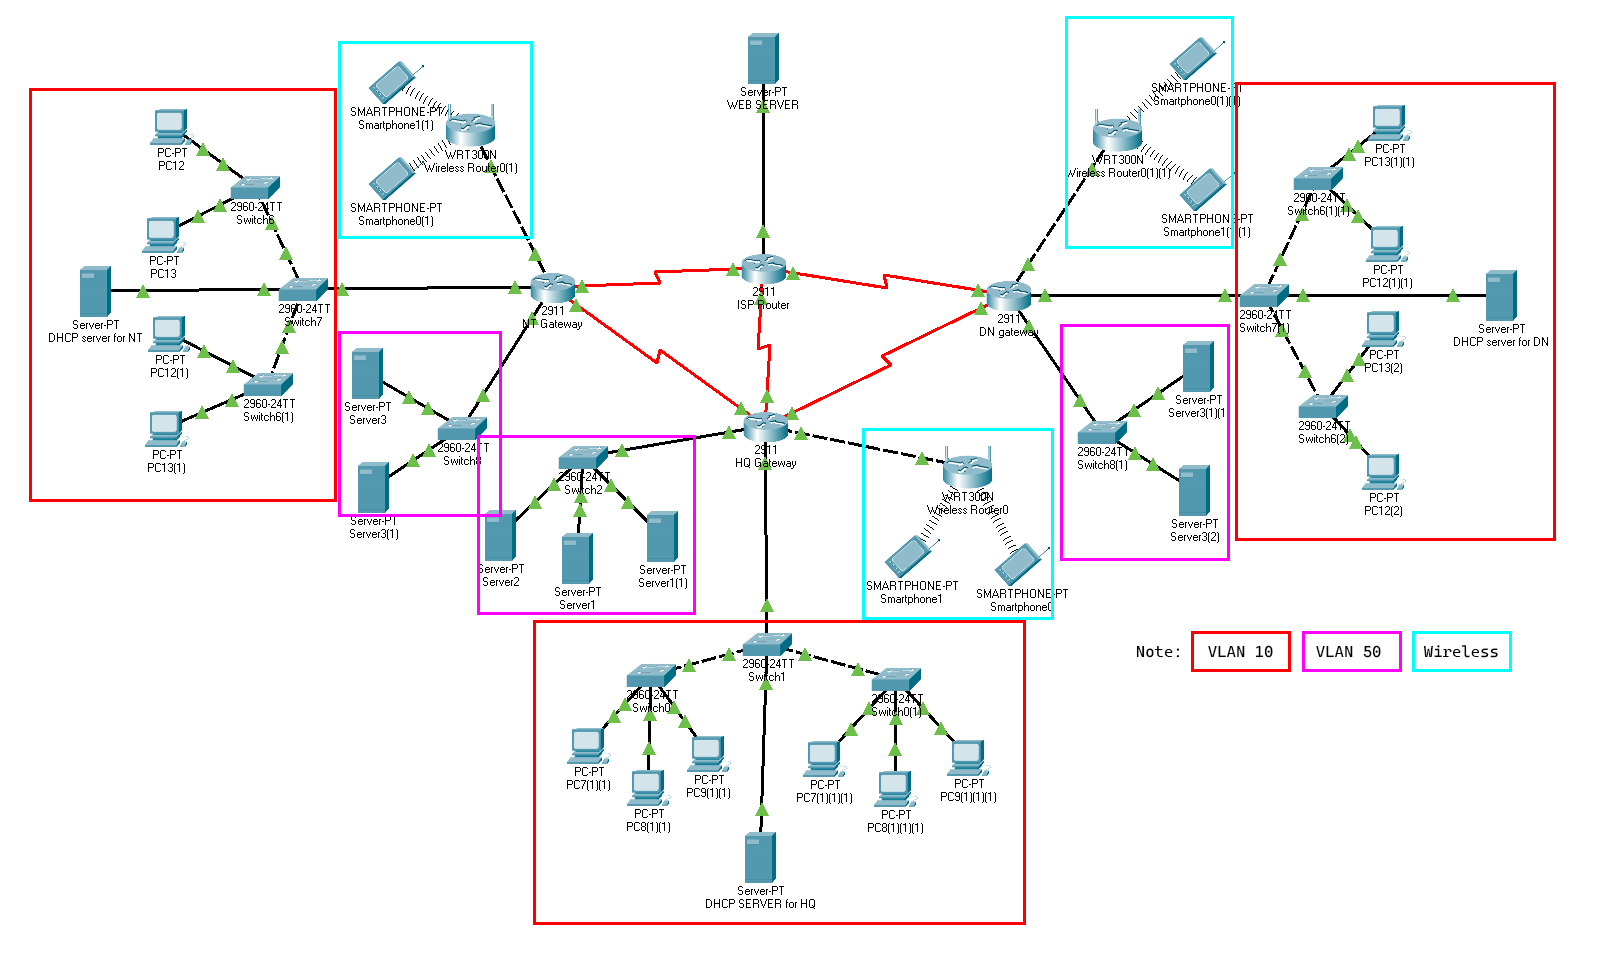
\includegraphics[width=0.8\textwidth]{./assets/pkt1.png}
  \caption{Topological diagram of the whole network}
\end{figure}

\textbf{Note:} This diagram does not contain all the network devices due to the poor runtime optimization of Packet Tracer.
This diagram is scaled down, however the principle and structure of the network should still hold.

\subsection{Switch and VLAN Configuration}
Here, we provide a sample configuration for the HQ.
For the switches in \textbf{VLAN 10}, we configure as follows.

First, we define \textbf{VLAN 10} using the CLI\@.
\begin{code}{Tcl}
  en
  conf t
  vlan 10
  name WorkStationHQ
  int range f0/1-24
  sw mode access
  sw access vlan 10
  int GigabitEthernet0/1
  sw mode access
  sw access vlan 10
  sw mode trunk
  exit
  end
\end{code}

Then, to have the switch provide DHCP service, we use the following commands.
\begin{code}{Tcl}
  en
  conf t
  int range f0/1-24
  sw mode trunk
  int range GigabitEthernet0/1-2
  sw mode access
  sw access vlan 10
  exit
  end
\end{code}

\begin{figure}[H]
  \centering
  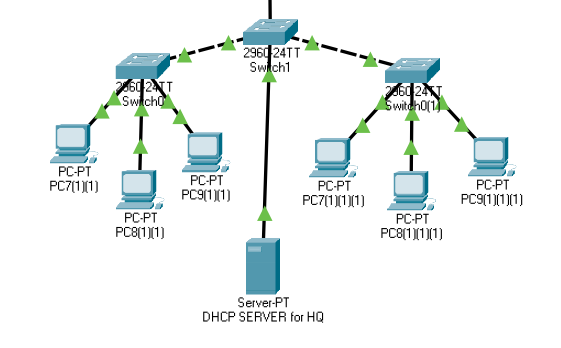
\includegraphics[width=0.8\textwidth]{./assets/pkt2.png}
  \caption{VLAN 10 setup of HQ}
\end{figure}

Now we will configure \textbf{VLAN 50}.
\begin{code}{Tcl}
  en
  conf t
  vlan 50
  name ServerHQ
  int range f0/1-24
  sw mode access
  sw access vlan 50
  int GigabitEthernet0/1
  sw mode access
  sw access vlan 50
  exit
  end
\end{code}

And that is all for the configurations of the network at HQ\@.
The same procedure applies with NT and DN branches.
We only need to change name and interface range.

\subsection{Wireless Router Configuration}
We connect to the default gateway address of the AP to begin configuration.
This address is usually 10.0.1.1, but it can also change if the device has subnet discovery.

\begin{figure}[H]
  \centering
  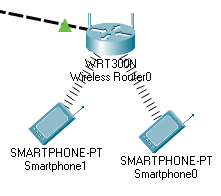
\includegraphics[width=0.4\textwidth]{./assets/ap1.png}
  \caption{Wireless router setup at HQ}
\end{figure}

Then we configure the AP using its GUI\@.
We set the IP address of the AP and the subnet mask as in the picture.
Then we enable the DHCP server, set the start IP address and the maximum number of users.

\begin{figure}[H]
  \centering
  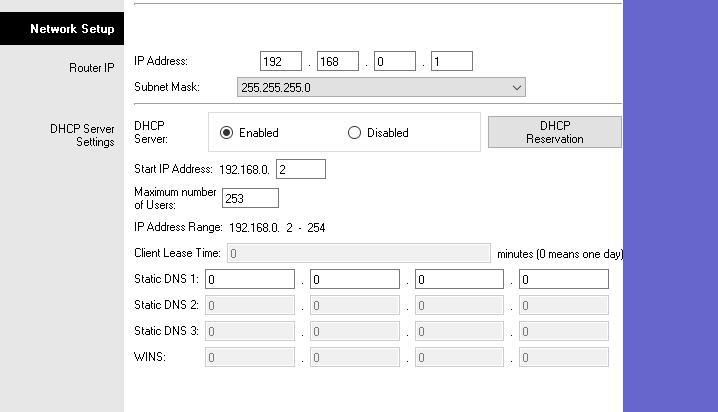
\includegraphics[width=0.8\textwidth]{./assets/wifi1.png}
  \caption{Wireless router setup for HQ}
\end{figure}

And that is the DHCP configuration at the HQ\@.
The same procedure applies with NT and DN branches.

\subsection{OSPF Protocol Setup}
With the use of OSPF protocol, we can manage the connection between the HQ and the branches.

We use the following commands for the gateway routers at HQ, 2 branches and the ISP router.
\begin{code}{Tcl}
  en
  conf t
  router ospf ID
  area AREA
\end{code}
where ID depends on the area.

We assign AREA = 0 as these routers are of the backbone area; ID = 1 for the HQ, 2 for the NT branch, and 3 for the DN branch.

\begin{figure}
  \centering
  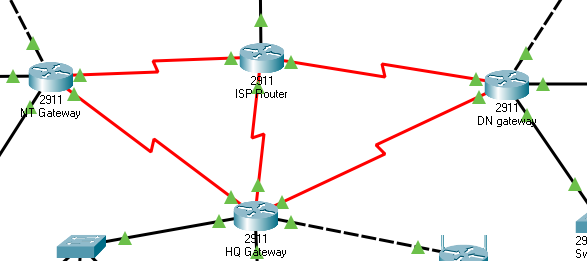
\includegraphics{./assets/core.png}
  \caption{Core network devices}
\end{figure}

\subsection{Security Setup}
In order to restrict the activity at the APs, we use access control list (ACL) to prevent a ping from reaching hosts on other area networks.

We will use the following commands for the 3 gateway routers of the bank.

\begin{code}{Tcl}
  en
  conf t
  ip access-list standard BBBank
  deny 10.0.1.2 0.0.0.0
  deny 10.1.1.2 0.0.0.0
  deny 10.2.1.2 0.0.0.0
  permit 10.0.0.0 0.255.255.255
  deny any
  exit
\end{code}

We continue by applying the ACL to the workstations

\begin{code}{Tcl}
  int GigabitEthernet0/0
  ip access-group BBBank out
  exit
\end{code}

Now we apply the ACL to the servers

\begin{code}{Tcl}
  int GigabitEthernet0/1
  ip access-group BBBank out
  exit
\end{code}

With that done, we can save this config

\begin{code}{Tcl}
  copy running-config startup-config
  write
\end{code}

We will now verify our configuration on ACL\@.

Firstly, we check the router's interface access-list policy

\begin{figure}[H]
  \centering
  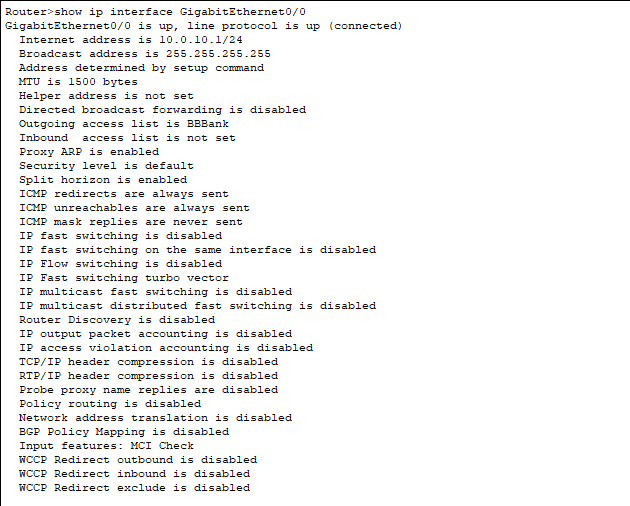
\includegraphics[width=0.8\textwidth]{./assets/acl1.png}
  \caption{ACL policy for the workstations at HQ}
\end{figure}

\begin{figure}[H]
  \centering
  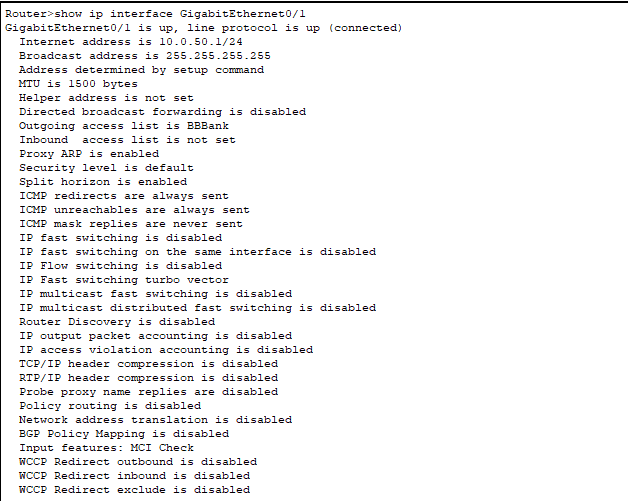
\includegraphics[width=0.8\textwidth]{./assets/acl2.png}
  \caption{ACL policy for the servers at HQ}
\end{figure}

Then we check the ACL group conditions

\begin{figure}[H]
  \centering
  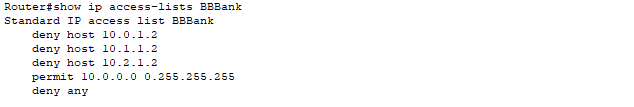
\includegraphics[width=0.8\textwidth]{./assets/acl3.png}
  \caption{IP access list of group BBBank}
\end{figure}


\section{System Tests}
\subsection{Ping Test}
% TODO

\subsection{Traceroute Test}
% TODO

\subsection{MAC Address Table and OSPF IP Table}
% TODO


\section{Results and Conclusions}
\subsection{Re-evaluation of the design}
\subsubsection{Reliability}
\begin{itemize}
    \item The message sent by network devices are receivable to the receivers.
    \item Our system might have packet loss. This might be occurred in the first route or ping because the network need to fill the MAC table of the switch. After this time, our system will deliver packets more easier with less packet loss.
\end{itemize}

\subsubsection{Easy to Upgrade}
\begin{itemize}
    \item Each subnet in a single networkcan provide up to 253 users, so our system can add and remove devices easily.
    \item When we want to add new branch to the network, we just add and configure new router corresponding to that branch. Then, connect to Headquarter router through WAN links.
\end{itemize}

\subsubsection{Diversity of Supporting Software}
Not only the Ethernet connection, our network system also provide wireless router for the wireless devices to access the Internet.

\subsubsection{Scalability}
\begin{itemize} 
        \item The use of network equipment from Cisco 
helps us to have better technical support, more stable equipment, and especially in
Cisco products that are often integrated, available new technologies.
    \item For the problem of bandwidth, with the increment rate of 20\% per 5 years so when we will safety factor of 20\% to make sure the network can have good performance for the next 10 years.
\end{itemize}

\subsubsection{Safety}
\begin{itemize}
    \item Support the mechanism to restrict IP address to come in and out of the Internet
    \item Servers are placed in a separate switch with their own VLANs and they connect to gateway routers through a separate port. Since this, our system can implement network configurations to enhance the network's security more conveniently.
    \item Providing security for wireless network by  applying ACL tables to limit the access from wireless devices to other devices
    \item Applying mechanism to prevent the wireless devices ping to other devices.    
    \item Sensitive data is kept confidential when there are packet theft attacks
\end{itemize}

\subsection{Remaining Problems}
\subsubsection{Security}
\begin{itemize}
    \item Although the ACL limit the IP from wireless access to ping other devices, this can also restrict the inter Network to receive message when the servers ping to the Internet
    \item The wifi password might be easy to guess

\end{itemize}

\subsubsection{Scalability}
\begin{itemize}
    \item Our network system can support up to 15 branches, so in the future, if the bank have more branches, there should be another enhancement in the network to adapt the scalability of the bank.
    \item Serial link for inter-branch may cause bottleneck problem when the bank grower bigger.

\end{itemize}

\subsection{Development Orientation}
\begin{itemize}
    \item Enhance security of the network to protect customer's data.
    \item Implement the ping from the Inter Network to Web server
    \item Conduct a detailed actual survey of the lines, structure of the wall and floor to
install the equipment
\item Use professional security measures, build a network security room to detect and
resolve situations in real time
\item Find the ways to improve the network when the bank grow bigger with the lowest cost with the good performance. A bank usually have a long life span, so we need to make the network to have a long life span as most as possible with the easiest maintenance.
\end{itemize}


\printbibliography[heading=bibintoc]

\end{document}
